%\setcounter{chapter}{5}
%\chapter{HÀM SỐ VÀ ĐỒ THỊ CỦA HÀM SỐ $y=ax^2$ ($a \neq  0$) VÀ PHƯƠNG TRÌNH BẬC HAI MỘT ẨN}
\section{HÀM SỐ VÀ ĐỒ THỊ CỦA HÀM SỐ $y=ax^2$ ($a \neq  0$)} % Tên bài
\subsection{Kiến thức trọng tâm}
\subsubsection{Hàm số $y=ax^2$ $(a \neq 0)$}
Hàm số xác định với mọi giá trị $x$ thuộc $\mathbb{R}$.
%%%%%%%Ví dụ 1
\begin{vd}%[SGK Chân Trời Sáng Tạo T9]%[Dự án EX-9-Đề Cương Toán 9]%[Thảo Thảo]%[9D6N1-1]
\begin{enumerate}
    \item Trong các hàm số sau, hàm số nào có dạng $y=ax^2$ ($a \neq 0$)?\\
    \centerline{$y=2x$; $y=3x^2$; $y=0x^2$; $y=-\dfrac{x^2}{4}$.}
    \item Xác định hệ số của $x^2$ trong các hàm số sau: $y=2x^2$; $y=-0{,}25x^2$; $y=\dfrac{1}{2}x^2$.
\end{enumerate}
\loigiai{
\begin{enumerate}
    \item Các hàm số có dạng $y=ax^2$ ($a \neq 0$) là
    \begin{itemize}
        \item $y=3x^2$ với $a=3$.
        \item $y=-\dfrac{x^2}{4}$ với $a=-\dfrac{1}{4}$.
    \end{itemize}
    \item Hệ số của $x^2$ trong hàm số
    \begin{itemize}
        \item $y=2x^2$ là $2$.
        \item $y=-0{,}25x^2$ là $-0{,}25$.
        \item $y=\dfrac{1}{2}x^2$ là $\dfrac{1}{2}$.
    \end{itemize}
\end{enumerate}
}
\end{vd}
%%%%%%%Ví dụ 2
\begin{vd}%[SGK Cánh Diều T9] %[Thảo Thảo, Dự án EX-9-Đề Cương Toán 9]%[9D6N2-1]
    Cho hàm số $y=4x^2$. Tính giá trị của $y$ khi
    \begin{enumerate}
        \item $x=0$.
        \item $x=2$.
        \item $x=-2$.
    \end{enumerate}
    \loigiai{
    \begin{enumerate}
        \item Thay $x=0$ vào công thức $y=4x^2$ ta được $y=4 \cdot 0^2=0$.
        \item Thay $x=2$ vào công thức $y=4x^2$ ta được $y=4 \cdot 2^2=16$.
        \item Thay $x=-2$ vào công thức $y=4x^2$ ta được $y=4 \cdot (-2)^2=16$.
    \end{enumerate}
    }
\end{vd}
%%%%%%%Ví dụ 3
\begin{vd}
    Cho hàm số $y=f(x)=-x^2$. Tính $f(1)$; $f(-1)$; $f(3)$.
    \loigiai{
    $f(1)=-1^2=-1$.\\
    $f(-1)=-(-1)^2=-1$.\\
    $f(3)=-3^2=-9$.
    }
\end{vd}
%%%%%%%%%%Ví dụ 4
\begin{vd}%[SGK Chân Trời Sáng Tạo T9]%[Dự án EX-9-Đề Cương Toán 9]%[Thảo Thảo]%[9D6N3-1]
    Gọi $x$ (\text{cm}) là chiều dài cạnh của một viên gạch lát nền hình vuông.
    \begin{enumerate}
        \item Viết công thức tính diện tích $S$ ($\text{cm}^2$) của viên gạch đó theo $x$.
        \item Tính $S$ khi $x=20$; $x=30$; $x=60$.
    \end{enumerate}
    \loigiai{
    \begin{enumerate}
        \item Công thức tính diện tích $S$ ($\text{cm}^2$) của viên gạch là $S(x)=x^2$.
        \item Với $x=20$ thì $S(20)=20^2=400$.\\
        Với $x=30$ thì $S(30)=30^2=900$.\\
        Với $x=60$ thì $S(60)=60^2=3\,600$.\\
    \end{enumerate}
    }
\end{vd}
\subsubsection{Bảng giá trị của hàm số $y=ax^2$ $(a \neq 0)$}
\begin{tomtat}
    Với hàm số $y=ax^2$ ($a \neq 0$) ta có
    \begin{itemize}
        \item Nếu $a>0$ thì $y>0$ với mọi $x \neq 0$; $y=0$ khi $x=0$.
        \item Nếu $a < 0$ thì $y<0$ với mọi $x \neq 0$; $y=0$ khi $x=0$.
    \end{itemize}
\end{tomtat}
\begin{vd}%[SGK Chân Trời Sáng Tạo T9]%[Dự án EX-9-Đề Cương Toán 9]%[Thảo Thảo]%[ID]
    Cho hàm số $y=\dfrac{1}{2}x^2$. Hoàn thành bảng giá trị sau
    \begin{center}
        \begin{tabular}{|c|c|c|c|c|c|} 
					\hline
					$x$ & $-4$ & $-2$ & $0$ & $2$ & $4$  \\ 
					\hline
					\parbox[c][1cm][c]{0cm}{}
					$y=\dfrac{1}{2}x^2$ &  &  & &  &  \\ 
					\hline
		\end{tabular} \hspace{1.2cm}
    \end{center}
    \loigiai{
    \begin{center}
        \begin{tabular}{|c|c|c|c|c|c|} 
					\hline
					$x$ & $-4$ & $-2$ & $0$ & $2$ & $4$  \\ 
					\hline
					\parbox[c][1cm][c]{0cm}{}
					$y=\dfrac{1}{2}x^2$ & $8$ & $2$ & $0$ & $2$ & $8$ \\ 
					\hline
		\end{tabular} \hspace{1.2cm}
    \end{center}
    }
\end{vd}			
\begin{vd}%[SGK Chân Trời Sáng Tạo T9]%[Dự án EX-9-Đề Cương Toán 9]%[Thảo Thảo]%[9D6H1-2]
    Một vật rơi tự do từ độ cao $125$ m so với mặt đất. Quãng đường chuyển động $s$ (m) của vật phụ thuộc vào thời gian $t$ (giây) được cho bởi công thức $s=5t^2$.
    \begin{enumerate}
        \item Sau $2$ giây, vật này cách mặt đất bao nhiêu mét? Tương tự, sau $3$ giây, vật cách mặt đất bao nhiêu mét?
        \item Sau bao lâu thì vật này tiếp đất?
    \end{enumerate}
    \loigiai{
    \begin{enumerate}
        \item Thay $t=2$ vào công thức $s=5t^2$ ta được $s=5 \cdot 2^2=20$.\\
        Vậy sau $2$ giây, vật cách mặt đất $125-20=105$ m.\\
        Thay $t=3$ vào công thức $s=5t^2$ ta được $s=5 \cdot 3^2=45$.\\
        Vậy sau $3$ giây, vật cách mặt đất $125-45=80$ m.
        \item Để vật tiếo đất thì quãng đường vật di chuyển được là $125$ m. Thay $s=125$ vào công thức $s=5t^2$ ta được\\
        \centerline{$125=5t^2$ suy ra $t^2=15$ hay $t=5$ (với $t>0$)}\\
        Vậy sau $5$ giây thì vật tiếp đất.
    \end{enumerate}
    }
\end{vd}
\subsubsection{Đồ thị của hàm số $y=ax^2$ $(a \neq 0)$}
\begin{tomtat}
    Đồ thị của hàm số $y=ax^2$ ($a \neq 0$) là một đường cong đi qua gốc toạ độ, nhận trục tung làm trục đối xứng. Đường cong đó được gọi là một parabol đỉnh $O$.
\begin{itemize}
    \item Nếu $a > 0$ thì đồ thị nằm phía trên trục hoành, $O$ là điểm thấp nhất của đồ thị.
    \item Nếu $a < 0$ thì đồ thị nằm phía dưới trục hoành, $O$ là điểm cao nhất của đồ thị.
\end{itemize}
Để vẽ đồ thị hàm số $y=ax^2$ ($a \neq 0$) ta thực hiện các bước sau
    \begin{itemize}
        \item Lập bảng giá trị của hàm số với một số giá trị của $x$ (thường lấy $5$ giá trị gồm $0$ và hai cặp giá trị đối nhau).
        \item Trên mặt phẳng toạ độ $Oxy$, đánh dấu các điểm $(x;y)$ trong bảng giá trị (gồm điểm $(0;0)$ và hai cặp điểm đối xứng nhau qua trục $Oy$).
        \item Vẽ đường parabol đi qua các điểm vừa được đánh dấu.
    \end{itemize}
\end{tomtat}
\begin{vd}%[SGK Chân Trời Sáng Tạo T9]%[Dự án EX-9-Đề Cương Toán 9]%[Thảo Thảo]%[9D6V1-2]
    Vẽ đồ thị của hàm số $y=2x^2$.
    \loigiai{
    Bảng giá trị
    \begin{center}
        \begin{tabular}{|c|c|c|c|c|c|} 
					\hline
					$x$ & $-2$ & $-1$ & $0$ & $1$ & $2$  \\ 
					\hline
					\parbox[c][1cm][c]{0cm}{}
					$y=2x^2$ & $8$ & $2$ & $0$ & $2$ & $8$ \\ 
					\hline
		\end{tabular} \hspace{1.2cm}
    \end{center}
    Đồ thị hàm số $y=2x^2$
    \begin{center}
        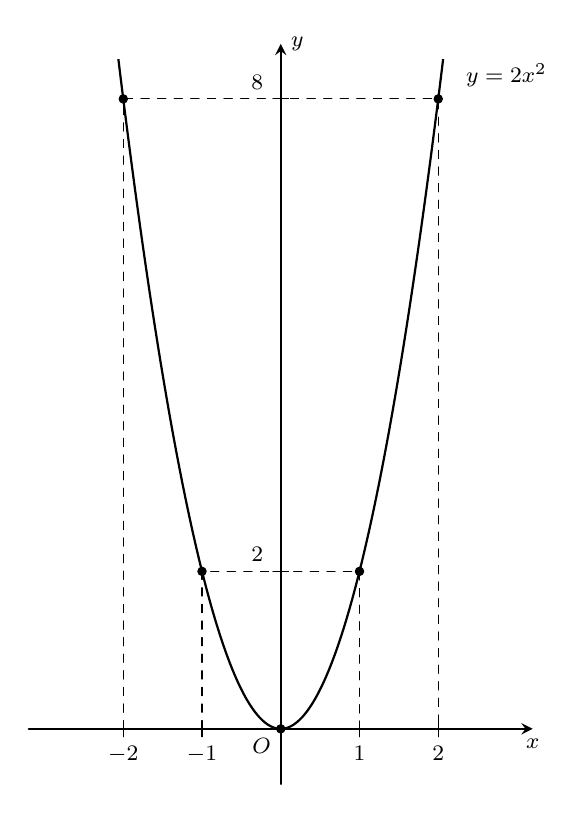
\begin{tikzpicture}[scale=1, font=\footnotesize, line join=round, line cap=round, >=stealth]
					% Kích thước trục
					\def\xmin{-3}\def\xmax{3}\def\ymin{-0.5}\def\ymax{8.5}
					
					% Vẽ hai trục toạ độ
					\draw[thick,->] (\xmin-0.2,0)--(\xmax+0.2,0) node[below] {\footnotesize $x$};
					\draw[thick, ->] (0,\ymin-0.2)--(0,\ymax+0.2) node[right] {$y$};
					
					% Kí hiểu điểm trên trục
					\draw (0,0) node [below left] {\footnotesize $O$};
					\foreach \x in {-2,-1,1,2}\draw (\x,0.1)--(\x,-0.1) node [below] {\footnotesize $\x$};
					\foreach \y in {2,8}\draw (0.1,\y)--(-0.1,\y) node [above left] {\footnotesize $\y$};
					\draw[fill=black] (2,8) circle (1.5pt);
					\draw[fill=black] (-2,8) circle (1.5pt);
					\draw[fill=black] (-1,2) circle (1.5pt);
					\draw[fill=black] (1,2) circle (1.5pt);
					\draw[fill=black] (0,0) circle (1.5pt);
					\draw[dashed] (-1,0)--(-1,2)--(1,2)--(1,0);
					\draw[dashed] (-2,0)--(-2,8)--(2,8)--(2,0);
					
					% Kí hiệu đồ thị
					\draw (3.5,8.3) node [left] {\footnotesize $y=2x^2$};
					
					% Vẽ đồ thị hàm số
					\clip (\xmin,\ymin) rectangle (\xmax,\ymax);
					\draw[thick, smooth,samples=100,domain=\xmin:\xmax] plot (\x,{2*(\x)^2});
				\end{tikzpicture}
    \end{center}
    }
\end{vd}
\begin{vd}%[SGK Chân Trời Sáng Tạo T9]%[Dự án EX-9-Đề Cương Toán 9]%[Thảo Thảo]%[9D6V2-2]
    Động năng (tính bằng $J$) của một quả bưởi nặng $1$ kg rơi với tốc độ $v$ ($\text{m}/\text{s}$) được tính bằng công thức $K=\dfrac{1}{2}v^2$.
    \begin{enumerate}
        \item Tính động năng của quả bưởi đạt được khi nó rơi với tốc độ $3$ m/s, $4$ m/s.
        \item Tính tốc độ rơi của quả bưởi tại thời điểm quả bưởi đạt được động năng $32$ $J$.
    \end{enumerate}
    \loigiai{
    \begin{enumerate}
        \item Thay $v=3$ vào công thức $K=\dfrac{1}{2}v^2$ ta được $K=\dfrac{1}{2}\cdot 3^2=4{,}5$.\\
        Vậy quả bưởi rơi với tốc độ $3$ m/s thì có động năng là $4{,}5$ $J$.\\
        Thay $v=4$ vào công thức $K=\dfrac{1}{2}v^2$ ta được $K=\dfrac{1}{2}\cdot 4^2=8$.\\
        Vậy quả bưởi rơi với tốc độ $4$ m/s thì có động năng là $8$ $J$.
        \item Thay $K=32$ vào công thức $K=\dfrac{1}{2}v^2$ ta được \\
        \centerline{$32=\dfrac{1}{2}v^2$ suy ra $v^2=64$ hay $v=8$ ($v>0$)} \\
        Vậy quả bưởi rơi với tốc độ $8$ m/s thì có động năng là $32$ $J$.
    \end{enumerate}
    }
\end{vd}
\subsection{Bài tập}
\begin{dang}
    {Tính giá trị hàm số tại một điểm cho trước}
    Ta thay giá trị của $x$ vào công thức của hàm số để tìm $y$.
\end{dang}

\begin{bt}%[SGK Chân Trời Sáng Tạo T9]%[Dự án EX-9-Đề Cương Toán 9]%[Thảo Thảo]%[9D6H2-1]
    Lập bảng giá trị của hàm số $y=\dfrac{1}{4}x^2$ và $y=-\dfrac{1}{4}x^2$ với $x$ lần lượt bằng $-4$; $-2$; $0$; $2$; $4$.
    \loigiai{
    Bảng giá trị
        \begin{center}
        \begin{tabular}{|c|c|c|c|c|c|} 
					\hline
					$x$ & $-4$ & $-2$ & $0$ & $2$ & $4$  \\ 
					\hline
					\parbox[c][1cm][c]{0cm}{}
					$y=\dfrac{1}{4}x^2$ & $4$ & $1$ & $0$ & $1$ & $4$ \\ 
					\hline
                    \parbox[c][1cm][c]{0cm}{}
					$y=-\dfrac{1}{4}x^2$ & $-4$ & $-1$ & $0$ & $-1$ & $-4$ \\ 
                    \hline
		\end{tabular} \hspace{1.2cm}
    \end{center}
    }
\end{bt}

\begin{bt}%[SGK Cánh Diều T9]%[Dự án EX-9-Đề Cương Toán 9]%[Thảo Thảo]%[9D6H3-1]
    Cho hàm số $y=\dfrac{1}{3}x^2$. 
    \begin{enumerate}
        \item Tìm giá trị của $y$ tương ứng với giá trị của $x$ trong bảng sau
        \begin{center}
        \begin{tabular}{|c|c|c|c|c|c|c|c|} 
					\hline
					$x$ & $-3$ & $-2$ & $-1$ & $0$ & $1$ & $2$  & $3$\\ 
					\hline
					\parbox[c][1cm][c]{0cm}{}
					$y=\dfrac{1}{3}x^2$ & $?$ & $?$ & $?$ & $?$ & $?$ & $?$ &$?$\\ 
					\hline
		\end{tabular} \hspace{1.2cm}
    \end{center}
        \item Tìm những điểm thuộc đồ thị của hàm số có hoành độ bằng $-6$; $10$.
        \item Tìm những điểm thuộc đồ thị của hàm số có tung độ bằng $27$.
    \end{enumerate}
        \loigiai{
        \begin{enumerate}
            \item Ta có bảng sau
            \begin{center}
        \begin{tabular}{|c|c|c|c|c|c|c|c|} 
					\hline
					$x$ & $-3$ & $-2$ & $-1$ & $0$ & $1$ & $2$  & $3$\\ 
					\hline
					\parbox[c][1cm][c]{0cm}{}
					$y=\dfrac{1}{3}x^2$ & $3$ & $\dfrac{4}{3}$ & $\dfrac{1}{3}$ & $0$ & $\dfrac{1}{3}$ & $\dfrac{4}{3}$ &$3$\\ 
					\hline
		\end{tabular} \hspace{1.2cm}
    \end{center}
    \item Với $x=6$ thì $y=\dfrac{1}{3} \cdot 6^2=12$.\\
    Với $x=10$ thì $y=\dfrac{1}{3} \cdot 10^2=\dfrac{100}{3}$.\\
    Vậy các điểm cần tìm là $(6;12)$, $\left(10;\dfrac{100}{3}\right)$.
    \item Với $y=27$ ta có $27=\dfrac{1}{3}x^2$, suy ra $x=9$ hoặc $x=-9$.\\
    Vậy các điểm cần tìm là $(9;27)$, $(-9;27)$.
        \end{enumerate}
        }
\end{bt}
\begin{dang}
    {Vẽ đồ thị hàm số $y=ax^2$ $(a \neq 0)$.}
    Để vẽ đồ thị hàm số $y=ax^2$ ($a \neq 0$) ta thực hiện các bước sau
    \begin{itemize}
        \item Lập bảng giá trị của hàm số với một số giá trị của $x$ (thường lấy $5$ giá trị gồm $0$ và hai cặp giá trị đối nhau).
        \item Trên mặt phẳng toạ độ $Oxy$, đánh dấu các điểm $(x;y)$ trong bảng giá trị (gồm điểm $(0;0)$ và hai cặp điểm đối xứng nhau qua trục $Oy$).
        \item Vẽ đường parabol đi qua các điểm vừa được đánh dấu.
    \end{itemize}
\end{dang}

\begin{bt}%[SGK Chân Trời Sáng Tạo T9]%[Dự án EX-9-Đề Cương Toán 9]%[Thảo Thảo]%[9D6V3-2]
    Cho hàm số $y=-x^2$.
    \begin{enumerate}
        \item Lập bảng giá trị của hàm số.
        \item Vẽ đồ thị hàm số.
    \end{enumerate}
    \loigiai{
    \begin{enumerate}
        \item Bảng giá trị
    \begin{center}
        \begin{tabular}{|c|c|c|c|c|c|} 
					\hline
					$x$ & $-2$ & $-1$ & $0$ & $1$ & $2$  \\ 
					\hline
					\parbox[c][1cm][c]{0cm}{}
					$y=-x^2$ & $-4$ & $-1$ & $0$ & $-1$ & $-4$ \\ 
					\hline
		\end{tabular} \hspace{1.2cm}
    \end{center}
    \item Đồ thị hàm số $y=-x^2$
    \begin{center}
        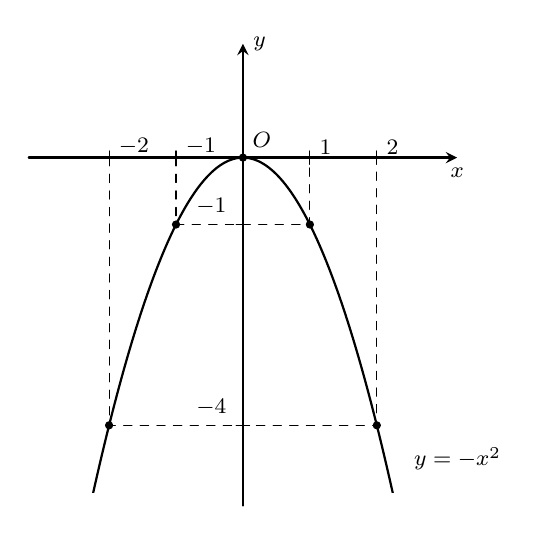
\begin{tikzpicture}[scale=0.85, font=\footnotesize, line join=round, line cap=round, >=stealth]
					% Kích thước trục
					\def\xmin{-3}\def\xmax{3}\def\ymin{-5}\def\ymax{1.5}
					
					% Vẽ hai trục toạ độ
					\draw[thick,->] (\xmin-0.2,0)--(\xmax+0.2,0) node[below] {\footnotesize $x$};
					\draw[thick, ->] (0,\ymin-0.2)--(0,\ymax+0.2) node[right] {$y$};
					
					% Kí hiểu điểm trên trục
					\draw (0,0) node [above right] {\footnotesize $O$};
					\foreach \x in {-2,-1,1,2}\draw (\x,0.1)--(\x,-0.1) node [above right] {\footnotesize $\x$};
					\foreach \y in {-1,-4}\draw (0.1,\y)--(-0.1,\y) node [above left] {\footnotesize $\y$};
					\draw[fill=black] (2,-4) circle (1.5pt);
					\draw[fill=black] (-2,-4) circle (1.5pt);
					\draw[fill=black] (-1,-1) circle (1.5pt);
					\draw[fill=black] (1,-1) circle (1.5pt);
					\draw[fill=black] (0,0) circle (1.5pt);
					\draw[dashed] (-1,0)--(-1,-1)--(1,-1)--(1,0);
					\draw[dashed] (-2,0)--(-2,-4)--(2,-4)--(2,0);
					
					% Kí hiệu đồ thị
					\draw (4,-4.5) node [left] {\footnotesize $y=-x^2$};
					
					% Vẽ đồ thị hàm số
					\clip (\xmin,\ymin) rectangle (\xmax,\ymax);
					\draw[thick, smooth,samples=100,domain=\xmin:\xmax] plot (\x,{-(\x)^2});
				\end{tikzpicture}
    \end{center}
    \end{enumerate}
    }
\end{bt}

\begin{bt}%[SGK Chân Trời Sáng Tạo T9]%[Dự án EX-9-Đề Cương Toán 9]%[Thảo Thảo]%[9D6V3-2]
    Cho hàm số $y=\dfrac{1}{2}x^2$.
    \begin{enumerate}
        \item Vẽ đồ thị của hàm số.
        \item Trong các điểm $A(-6;-8)$, $B(6;8)$, $C\left(\dfrac{2}{3};\dfrac{2}{9}\right)$, điểm nào thuộc đồ thị hàm số trên? 
    \end{enumerate}
    \loigiai{
    \begin{enumerate}
        \item Bảng giá trị
        \begin{center}
        \begin{tabular}{|c|c|c|c|c|c|} 
					\hline
					$x$ & $-4$ & $-2$ & $0$ & $2$ & $4$  \\ 
					\hline
					\parbox[c][1cm][c]{0cm}{}
					$y=\dfrac{1}{2}x^2$ & $8$ & $2$ & $0$ & $2$ & $8$ \\ 
					\hline
		\end{tabular} \hspace{1.2cm}
    \end{center}
    Vẽ đồ thị
    \begin{center}
        \begin{tikzpicture}[scale=0.65, font=\footnotesize, line join=round, line cap=round, >=stealth]
					% Kích thước trục
					\def\xmin{-4.5}\def\xmax{6}\def\ymin{-1}\def\ymax{8.5}
					
					% Vẽ hai trục toạ độ
					\draw[thick,->] (\xmin-0.2,0)--(\xmax+0.2,0) node[below] {\footnotesize $x$};
					\draw[thick, ->] (0,\ymin-0.2)--(0,\ymax+0.2) node[right] {$y$};
					
					% Kí hiểu điểm trên trục
					\draw (0,0) node [below left] {\footnotesize $O$};
					\foreach \x in {-4,-2,2,4}\draw (\x,0.1)--(\x,-0.1) node [below] {\footnotesize $\x$};
					\foreach \y in {2,8}\draw (0.1,\y)--(-0.1,\y) node [above left] {\footnotesize $\y$};
					\draw[fill=black] (4,8) circle (1.5pt);
					\draw[fill=black] (-4,8) circle (1.5pt);
					\draw[fill=black] (-2,2) circle (1.5pt);
					\draw[fill=black] (2,2) circle (1.5pt);
					\draw[fill=black] (0,0) circle (1.5pt);
					\draw[dashed] (-2,0)--(-2,2)--(2,2)--(2,0);
					\draw[dashed] (-4,0)--(-4,8)--(4,8)--(4,0);
					
					% Kí hiệu đồ thị
					\draw (6.6,8.3) node [left] {\footnotesize $y=\dfrac{1}{2}x^2$};
					
					% Vẽ đồ thị hàm số
					\clip (\xmin,\ymin) rectangle (\xmax,\ymax);
					\draw[thick, smooth,samples=100,domain=\xmin:\xmax] plot (\x,{(\x)^2/2});
				\end{tikzpicture}
    \end{center}
    \item Do $-8 \neq \dfrac{1}{2} \cdot (-6)^2$; $8 \neq \dfrac{1}{2} \cdot 6^2$ và $\dfrac{2}{9} = \dfrac{1}{2} \cdot \left(\dfrac{2}{3}\right)^2$ nên các điểm $A$, $B$ không thuộc đồ thị hàm số, điểm $C$ thuộc đồ thị hàm số.
    \end{enumerate}
    }
\end{bt}

\begin{bt}%[SGK Chân Trời Sáng Tạo T9]%[Dự án EX-9-Đề Cương Toán 9]%[Thảo Thảo]%[9D6V4-2]
    Cho hàm số $y=ax^2$ $(a \neq 0)$.
    \begin{enumerate}
        \item Tìm $a$, biết đồ thị của hàm số đi qua điểm $M(2;6)$.
        \item Vẽ đồ thị của hàm số với giá trị $a$ vừa tìm được.
        \item Tìm các điểm thuộc đồ thị trên có tung độ $y=9$.
    \end{enumerate}
    \loigiai{
    \begin{enumerate}
        \item Thay $x=2$; $y=6$ vào công thức $y=ax^2$ ta được\\
        \centerline{$6=a \cdot 2^2$ suy ra $a=\dfrac{3}{2}$.}
        \item Với $a=\dfrac{3}{2}$ ta có hàm số $y=\dfrac{3}{2}x^2$.\\
        Bảng giá trị
        \begin{center}
        \begin{tabular}{|c|c|c|c|c|c|} 
					\hline
					$x$ & $-2$ & $-1$ & $0$ & $1$ & $2$  \\ 
					\hline
					\parbox[c][1cm][c]{0cm}{}
					$y=\dfrac{3}{2}x^2$ & $6$ & $1{,}5$ & $0$ & $1{,}5$ & $6$ \\ 
					\hline
		\end{tabular} \hspace{1.2cm}
    \end{center}
    Vẽ đồ thị
    \begin{center}
        \begin{tikzpicture}[scale=0.8, font=\footnotesize, line join=round, line cap=round, >=stealth]
					% Kích thước trục
					\def\xmin{-3}\def\xmax{3}\def\ymin{-1}\def\ymax{6.5}
					
					% Vẽ hai trục toạ độ
					\draw[thick,->] (\xmin-0.2,0)--(\xmax+0.2,0) node[below] {\footnotesize $x$};
					\draw[thick, ->] (0,\ymin-0.2)--(0,\ymax+0.2) node[right] {$y$};
					
					% Kí hiểu điểm trên trục
					\draw (0,0) node [below left] {\footnotesize $O$};
					\foreach \x in {-2,-1,1,2}\draw (\x,0.1)--(\x,-0.1) node [below] {\footnotesize $\x$};
					\foreach \y in {1,6}\draw (0.1,\y)--(-0.1,\y) node [above left] {\footnotesize $\y$};
					\draw[fill=black] (2,6) circle (1.5pt);
					\draw[fill=black] (-2,6) circle (1.5pt);
					\draw[fill=black] (-1,1.5) circle (1.5pt);
					\draw[fill=black] (1,1.5) circle (1.5pt);
					\draw[fill=black] (0,0) circle (1.5pt);
					\draw[dashed] (-2,0)--(-2,6)--(2,6)--(2,0);
					\draw[dashed] (-1,0)--(-1,1.5)--(1,1.5)--(1,0);
					
					% Kí hiệu đồ thị
					\draw (4.2,6.3) node [left] {\footnotesize $y=\dfrac{3}{2}x^2$};
					
					% Vẽ đồ thị hàm số
					\clip (\xmin,\ymin) rectangle (\xmax,\ymax);
					\draw[thick, smooth,samples=100,domain=\xmin:\xmax] plot (\x,{3*(\x)^2/2});
				\end{tikzpicture}
    \end{center}
    \item Thay $y=9$ vào công thức $y=\dfrac{3}{2}x^2$ ta được \\
    \centerline{$9=\dfrac{3}{2}x^2$ suy ra $x^2=6$, do đó $x=\sqrt{6}$ hoặc $x=-\sqrt{6}$.}\\
    Vậy các điểm cần tìm là $(\sqrt{6};9)$; $(-\sqrt{6};9)$.
    \end{enumerate}
    }
\end{bt}

\begin{dang}
    {Ứng dụng của đồ thị hàm số $y=ax^2$ $(a \neq 0)$.}
    \begin{vd} %[Dự án EX-9-Đề Cương Toán 9]%[Thảo Thảo]%[9D6V1-3]
	Một chiếc ô tô đang chạy thì bắt đầu tăng tốc. Quãng đường đi được của chiếc ô tô đó kể từ khi bắt đầu tăng tốc được tính theo công thức: $s=t^{2}+16 t$ ($s$ tính bằng mét, $t$ tính bằng giây, $t>0$).
	\begin{enumerate}
		\item Tính quãng đường ô tô đó đi được sau $7$ giây kể từ khi bắt đầu tăng tốc.
		\item Ô tô đó mất bao lâu để đi được quãng đường $80$ m kể từ khi bắt đầu tăng tốc?
	\end{enumerate}
	\loigiai{
		\begin{enumerate}
			\item Quãng đường ô tô đó đi được sau $7$ giây kể từ khi bắt đầu tăng tốc là $7^2+16\cdot 7 = 161$ (m).
			\item Để đi được quãng đường $80$ m kể từ khi bắt đầu tăng tốc, nghĩa là ta có phương trình
			$$t^2 + 16t = 80.$$
            Suy ra $(t+8)^2=144$, do đó $t+8=12$ hoặc $t+8=-12$.\\
			Giải phương trình, ta được $t = 4$ (thỏa mãn); $t = -20$ (loại).\\
			Vậy sau $4$ giây thì ô tô đi được quãng đường $80$ m.
		\end{enumerate}
	}
\end{vd}
\end{dang}
\begin{bt}%[Dự án EX-9-Đề Cương Toán 9]%[Thảo Thảo]%[9D6V2-3]
	Một quả bóng được ném lên theo phương thẳng đứng từ mặt đất với vận tốc ban đầu là $14{,}7$ m/s. Khi bỏ qua sức cản của không khí, độ cao $h$ (m) của quả bóng so với mặt đất được tính theo thời gian $t$ (giây) bởi công thức $h(t) = -4{,}9t^2 + 14{,}7t$ $(t \geq 0)$.
	\begin{enumerate}
		\item Tìm thời điểm quả bóng đó có độ cao so với mặt đất là $9{,}8$ m.		
		\item Sau bao lâu thì quả bóng đó rơi tiếp đất? 	
	\end{enumerate}
	\loigiai{
		\begin{enumerate}
			\item Ta có thời điểm $t$ (giây) mà quả bóng đó có độ cao so với mặt đất là $9{,}8$ m là nghiệm của phương trình $-4{,}9t^2+14{,}7t = 9{,}8$ hay $-4{,}9t^2 + 14{,}7t - 9{,}8 = 0$.\\	
			Phương trình trên, ta được $t_1 = 1$ (thoả mãn); $t_2 = 2$ (thoả mãn).\\	
			Vậy vào thời điểm $t=1$ giây hoặc $t=2$ giây thì quả bóng đó có độ cao so với mặt đất là $9{,}8$ m.	
			\item Quả bóng đó rơi tiếp đất khi độ cao của nó bằng $0$. Từ đó, ta có phương trình
			$$ -4{,}9t^{2} + 14,7t = 0. $$
			Giải phương trình, ta được $t = 0$ (thỏa mãn) và $t = 3$ (thỏa mãn).\\
			Thời điểm $t=0$ là thời điểm ban đầu mà quả bóng đó chưa được ném đi.\\	
			Vậy sau $t=3$ giây thì quả bóng đó rơi chạm đất.
		\end{enumerate}
	}
\end{bt}

\begin{bt}%[Dự án EX-9-Đề Cương Toán 9]%[Thảo Thảo]%[9D6V3-3]
	Một vật rơi ở độ cao so với mặt đất là $200$ m. Quãng đường chuyển động $S$ (mét) của vật rơi phụ thuộc vào thời gian $t$ (giây) bởi công thức $S(t)=4t^2-100t+197$. Hỏi sau bao lâu vật này cách mặt đất $3$ m?
	\loigiai{
		Vật rơi ở độ cao so với mặt đất là $200$ m nên khi cách mặt đất $3$ m có nghĩa là quãng đường vật đó đã đi được là $200-3=197$ (m).\\
		Do đó 
		\allowdisplaybreaks
		\begin{eqnarray*}
			S(t) &=&197 \\
			4t^2-100t+197&=&197\\
			4t^2-100t&=&0\\
			4t(t-25)&=&0\\
			4t=0 \text{ hoặc } t-25&=&0\\
			t=0 \text{ (loại)} \text{ hoặc } t&=&25 \text{ (nhận).}
		\end{eqnarray*}
		Với điều kiện $t>0$ thì ta được $t=25$.\\
		Vậy sau $25$ giây thì vật cách mặt đất $3$ m.
	}
\end{bt}

\begin{bt}%[SBT Cánh Diều T9]%[Dự án EX-9-Đề Cương Toán 9]%[Thảo Thảo]%[9D6V4-3]
	Doanh thu $T$ (nghìn đồng) từ tiền bán vé trong ngày $1$ tháng $6$ của một rạp chiếu phim vối giá mỗi vé là $x$ (nghìn đồng) được tính theo công thức: $T = -10x^2 + 700x - 1$. Xác định giá vé bán trong ngày $1$ tháng $6$ của rạp chiếu phim đó, biết doanh thu từ tiền bán vé của ngày hôm đó là $12\,249$ nghìn đồng.
	\loigiai{
		Vì doanh thu từ tiền bán vé của ngày hôm đó là $12\,249$ nghìn đồng nên ta có phương trình
		$$-10x^2 + 700x - 1 = 12\,249 \text{ hay } 10x^2 - 700x + 12\,250 = 0.$$	
		Giải phương trình, ta được $x = 35$ (thỏa mãn).\\
		Do đó, giá vé  bán trong ngày $1$ tháng $6$ của rạp chiếu phim là $35$ nghìn đồng.
	}
\end{bt}

\begin{bt}%[Tham Khảo HK2 NH 24-25, TPHCM, Tp. Thủ Đức]%[Dự án EX-9-Đề Cương Toán 9]%[Thảo Thảo]%[9D6V5-3]
	Giả sử doanh thu $R(x)$ (nghìn đồng) của một cửa hàng bán phở trong một ngày có thể mô hình hóa bằng công thức $R(x) = x(220 - 4x)$ với $30 \leq x \leq 50$, trong đó $x$ (nghìn đồng) là giá tiền của một bát phở. Nếu muốn doanh thu của cửa hàng đạt $3$ triệu đồng trong một ngày thì giá bán của mỗi bát phở là bao nhiêu?
	\loigiai{
		Đổi đơn vị: $3$ triệu $= 3\,000$ nghìn đồng.\\
		Để doanh thu của cửa hàng đạt $3$ triệu đồng trong một ngày thì
		\allowdisplaybreaks
		\begin{eqnarray*}
			x(220 - 4x) &=& 3\,000 \\
			220x - 4x^2 &=& 3\,000\\
			-4x^2 + 220x - 3\,000 &=& 0\\
			x = 30 \text{ (nhận)} \text{ hoặc } x &=& 25 \text{ (loại).}
		\end{eqnarray*}
		Vậy nếu muốn doanh thu của cửa hàng đạt $3$ triệu đồng trong một ngày thì giá bán của mỗi bát phở là $30$ nghìn đồng.
	}
\end{bt}
\begin{bt}%[Tham Khảo HK2 NH 24-25, TPHCM, Tp. Thủ Đức]%[Dự án EX-9-Đề Cương Toán 9]%[Thảo Thảo]%[9D6V6-3]
	Giả sử số lượng cá trong một hồ nào đó tăng, giảm theo công thức
	$P=50\left(100+15t-t^2\right)$, $0\leq t\leq 15$. 
	Ở đây $P$ là số lượng cá trong hồ sau $t$ năm tính từ ngày $01$ tháng $01$ năm $2020$, khi lần đầu tiên số lượng cá trong hồ được ước tính. Hỏi theo mô hình này thì	
	\begin{enumerate}
		\item Vào thời điểm nào thì số lượng cá trong hồ sẽ là $7~500$ con?
		\item Vào thời điểm nào, số lượng cá trong hồ sẽ trở lại như thời điểm ban đầu vào ngày $01$ tháng $01$ năm $2020$?
	\end{enumerate}
	\loigiai
	{
		\begin{enumerate}
			\item Thay $P=7\,500$ vào $P=50\left(100+15t-t^2\right)$, $0\leq t\leq 15$.	\\	
			Ta được
			\begin{eqnarray*}
				50\left(100+15t-t^2\right)&=&7\,500\\
				-50t^2+750t-2\,500&=&0.
			\end{eqnarray*} 
			Giải phương trình trên ta được $t=10$ (nhận); $t=5$(nhận).\\
			Vậy vào năm $2025$; $2030$ thì số lượng cá trong hồ sẽ là $7~500$ con.
			\item Thời điểm $01$ tháng $01$ năm $2020$, ta có $t=0$.\\
			Suy ra $P=50\cdot 100=5\,000$ con.\\
			Do đó, để số lượng cá trong hồ sẽ trở lại như thời điểm ban đầu thì
			\allowdisplaybreaks
			\begin{eqnarray*}
				50\left(100+15t-t^2\right)&=&5\,000\\
				-50t^2 + 750t &=& 0\\
				t = 0 \text{ (loại)} \text{ hoặc } t &=& 15 \text{ (nhận).} 
			\end{eqnarray*}
			Vậy vào năm $2035$ số lượng cá trong hồ sẽ trở lại như thời điểm ban đầu vào ngày $01$ tháng $01$ năm $2020$.
		\end{enumerate}
	}
\end{bt} 

\begin{bt}%[SGK Chân Trời Sáng Tạo T9]%[Dự án EX-9-Đề Cương Toán 9]%[Thảo Thảo]%[9D6V7-3]
    Cho một hình lập phương có độ dài cạnh là $x$ (cm).
    \begin{enumerate}
        \item Viết công thức tính diện tích toàn phần $S$ của hình lập phương theo $x$.
        \item Lập bảng giá trị của hàm số $S$ khi $x$ lần lượt nhận các giá trị $\dfrac{1}{2}$; $1$; $\dfrac{2}{3}$; $2$; $3$.
        \item Tính độ dài cạnh của hình lập phương, biết $S=54$ cm$^2$.
    \end{enumerate}
    \loigiai{
    \begin{enumerate}
        \item $S=6x^2$.
        \item Bảng giá trị
        \begin{center}
        \begin{tabular}{|c|c|c|c|c|c|} 
					\hline
					$x$ & $\dfrac{1}{2}$ & $1$ & $\dfrac{2}{3}$ & $2$ & $3$  \\ 
					\hline
					\parbox[c][1cm][c]{0cm}{}
					$S=6x^2$ & $\dfrac{3}{2}$ & $6$ & $\dfrac{8}{3}$ & $24$ & $54$ \\ 
					\hline
		\end{tabular} \hspace{1.2cm}
    \end{center}
    \item Thay $S=54$ vào công thức $S=6x^2$ ta được $54=6x^2$, suy ra $x^2=9$ hay $x=3$ (do $x>0$).\\
    Vậy độ dài cạnh của hình lập phương là $3$ cm.
    \end{enumerate}
    }
\end{bt}

\begin{bt}%[SGK Kết Nối Tri Thức T9]%[Dự án EX-9-Đề Cương Toán 9]%[Thảo Thảo]%[9D6V8-3]
    Cho hình lăng trụ đứng có đáy là hình vuông cạnh $a$ (cm) và chiều cao $10$ cm.
    \begin{enumerate}
        \item Viết công thức tính thể tích $V$ của hình lăng trụ theo $a$ và tính giá trị của $V$ khi $a=2$ cm.
        \item Nếu độ dài cạnh đáy tăng lên hai lần thì thể tích của hình lăng trụ thay đổi thế nào?
    \end{enumerate}
    \loigiai{
    \begin{enumerate}
        \item $V=10a^2$. Khi $a=2$ thì $V=10 \cdot 2^2=40$ cm$^3$.
        \item Nếu độ dài cạnh đáy tăng lên hai lần thì thể tích của hình lăng trụ là \\
        $V_1=10 \cdot (2a)^2=4 \cdot 10a^2=4V$.\\
        Vậy thể tích hình lăng trụ tăng gấp $4$ lần.
    \end{enumerate}
    }
\end{bt}

\begin{bt}%[SGK Chân Trời Sáng Tạo T9]%[Dự án EX-9-Đề Cương Toán 9]%[Thảo Thảo]%[9D6V9-3]
    Khi gió thổi vuông góc vào cánh buồm của một con thuyền thì lực $F$ (N) của nó tỉ lệ thuận với bình phương tốc độ $v$ (m/s) của gió, tức là $F=av^2$ ($a$ là hằng số). Biết rằng khi tốc độ gió bằng $3$ m/s thì lực tác động lên cánh buồm bằng $180$ N.
    \begin{enumerate}
        \item Tính hằng số $a$.
        \item Với $a$ vừa tìm được, tính lực $F$ khi $v=15$ m/s và khi $v=26$ m/s.
        \item Biết rằng cánh buồm có thể chịu được một lực tối đa là $14580$ N, hỏi con thuyền có thể đi được trong gió bão với tốc độ gió $90$ km/h hay không?
    \end{enumerate}
    \loigiai{
    \begin{enumerate}
        \item Thay $a=3$ và $F=180$ vào công thức $F=av^2$ ta được: $180=a \cdot 3^2$ hay $a=20$.
        \item Với $a=20$ thì $F=20v^2$.
        \begin{itemize}
            \item Khi $v=15$ thì $F=20 \cdot 15^2=4\,500$ (N).
            \item Khi $v=26$ thì $F=20 \cdot 26^2=13\,520$ (N).
        \end{itemize}
        \item Đổi $90 \, \text{km/h}=25 \, \text{m/s}$.\\
        Với $v=25$ ta có $F=20 \cdot 25^2=12\,500$ (N).\\
        Ta thấy $12\,500<14\,580$ nên con thuyền có thể đi được trong gió bão với tốc độ gió $90$ km/h.
    \end{enumerate}
    }
\end{bt}

